\documentclass[tikz,border=12pt]{standalone}
\usepackage[T1]{fontenc}
\usepackage{mathpazo}
\usepackage{amsmath,amssymb}
\usetikzlibrary{arrows.meta, positioning, calc}

\definecolor{stblue}{HTML}{7B97AD}
\definecolor{rwgold}{HTML}{B8995E}
\definecolor{sage}{HTML}{7A9A7E}
\definecolor{dkbrown}{HTML}{3D3530}
\definecolor{wmgray}{HTML}{7B7067}
\definecolor{cream}{HTML}{F9F6F0}
\definecolor{border}{HTML}{D4C9B8}

\begin{document}
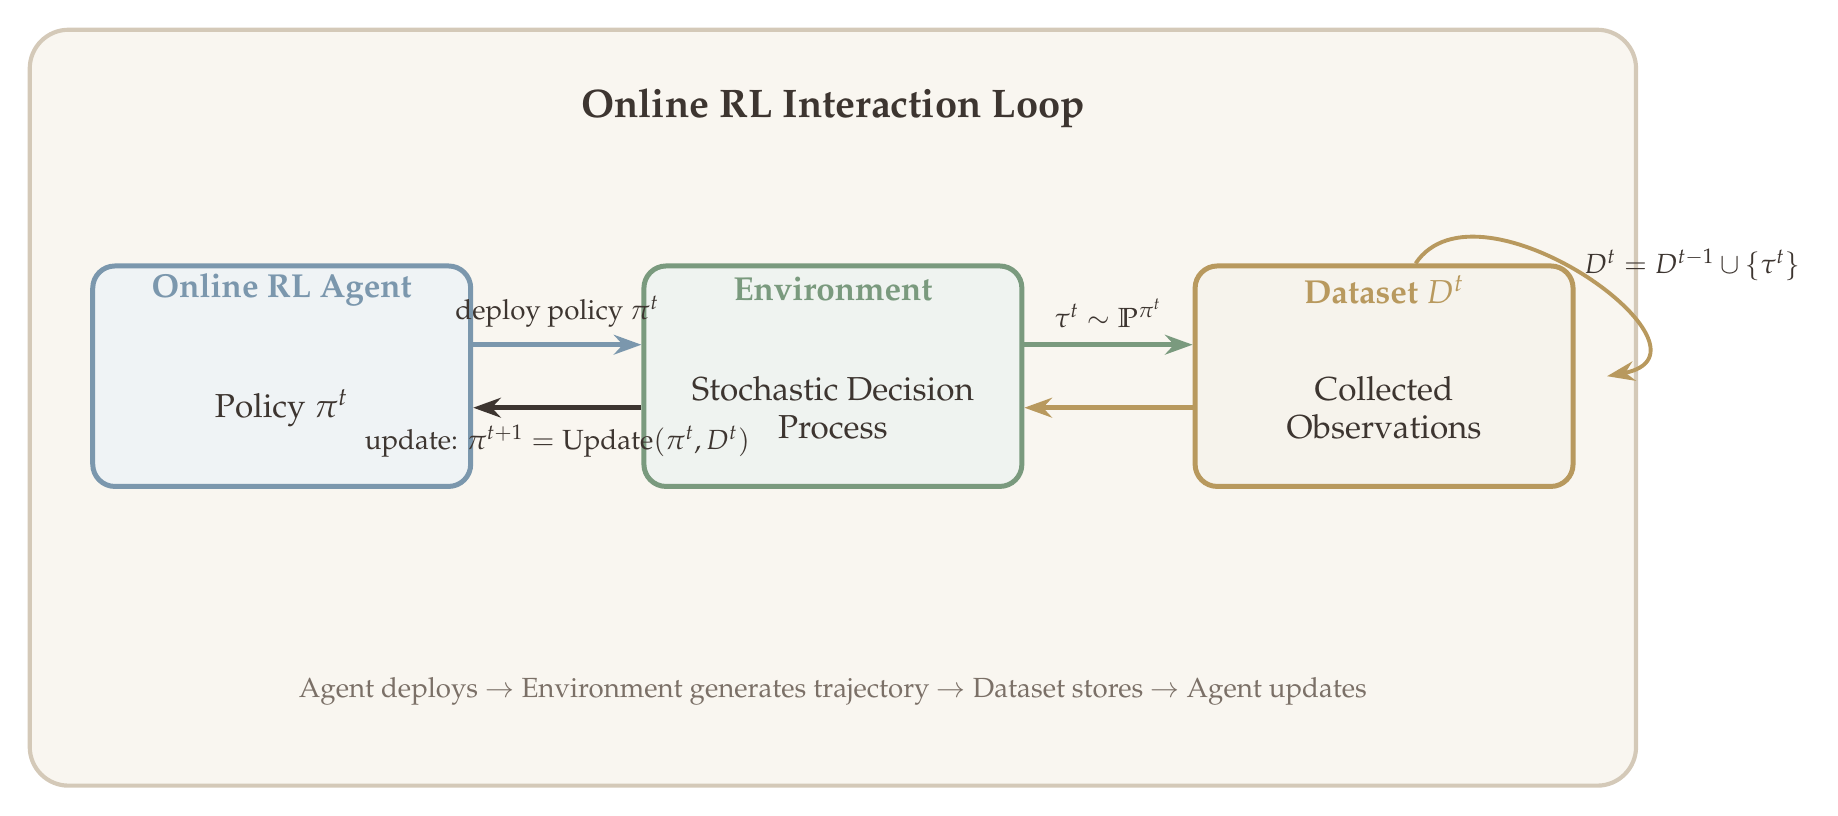
\begin{tikzpicture}[
  >={Stealth[length=3.5mm, width=2.5mm]},
  box/.style 2 args={
    draw=#1, line width=1.8pt, fill=#1!12, rounded corners=8pt,
    minimum width=48mm, minimum height=28mm,
    font=\large, text=dkbrown, align=center, inner sep=6pt},
  arr/.style={->, line width=1.8pt, dkbrown},
]

% Background canvas (~20cm x 9cm)
\fill[cream, rounded corners=14pt] (-1.2,-4.8) rectangle (19.2,4.8);
\draw[border, rounded corners=14pt, line width=1.5pt] (-1.2,-4.8) rectangle (19.2,4.8);

% Title
\node[font=\Large\bfseries, text=dkbrown] at (9.0,3.8)
  {Online RL Interaction Loop};

% === Box 1: Online RL Agent (stblue) ===
\node[box={stblue}{}] (agent) at (2.0,0.4) {};
\node[font=\large\bfseries, text=stblue] at (2.0,1.5) {Online RL Agent};
\node[font=\large, text=dkbrown] at (2.0,0.0) {Policy $\pi^t$};

% === Box 2: Environment (sage) ===
\node[box={sage}{}] (env) at (9.0,0.4) {};
\node[font=\large\bfseries, text=sage] at (9.0,1.5) {Environment};
\node[font=\large, text=dkbrown, align=center] at (9.0,0.0) {Stochastic Decision\\Process};

% === Box 3: Dataset (rwgold) ===
\node[box={rwgold}{}] (data) at (16.0,0.4) {};
\node[font=\large\bfseries, text=rwgold] at (16.0,1.5) {Dataset $D^t$};
\node[font=\large, text=dkbrown, align=center] at (16.0,0.0) {Collected\\Observations};

% === Top arrows: Agent -> Environment -> Dataset ===
\draw[arr, stblue, line width=1.8pt]
  ([yshift=4mm]agent.east) -- ([yshift=4mm]env.west)
  node[midway, above=2pt, font=\normalsize, text=dkbrown] {deploy policy $\pi^t$};

\draw[arr, sage, line width=1.8pt]
  ([yshift=4mm]env.east) -- ([yshift=4mm]data.west)
  node[midway, above=2pt, font=\normalsize, text=dkbrown] {$\tau^t \sim \mathbb{P}^{\pi^t}$};

% === Right-side self-arrow on Dataset ===
\draw[arr, rwgold, line width=1.4pt]
  ([xshift=4mm]data.north) .. controls +(0.8,1.2) and +(1.6,0.3) .. ([xshift=4mm]data.east)
  node[pos=0.45, right=3pt, font=\normalsize, text=dkbrown, align=left]
  {$D^t = D^{t-1} \cup \{\tau^t\}$};

% === Bottom arrow: Dataset -> Agent (update) ===
\draw[arr, rwgold, line width=1.8pt]
  ([yshift=-4mm]data.west) -- ([yshift=-4mm]env.east);
\draw[arr, dkbrown, line width=1.8pt]
  ([yshift=-4mm]env.west) -- ([yshift=-4mm]agent.east)
  node[midway, below=2pt, font=\normalsize, text=dkbrown, align=center]
  {update: $\pi^{t+1} = \mathrm{Update}(\pi^t, D^t)$};

% Extend bottom label to span the full return path
\node[font=\normalsize, text=wmgray] at (9.0,-3.6)
  {Agent deploys $\to$ Environment generates trajectory
   $\to$ Dataset stores $\to$ Agent updates};

\end{tikzpicture}
\end{document}
